% !TEX root = msc_thesis.tex

\mychapter{2}{Implementation} \label{chap:implementation}

asdf  sdfASd s s asd fdas
 asd dsfsdfdd

 dsfsadfa sfdas 

\section{ELASPIC pipeline}

\section{Homology modeling}

We used the MODELLER software package to perform all homology modeling.

``MODELLER uses simulated annealing cycles along with a minimal forcefield and spatial restraints -- generally Gaussian interatomic probability densities extracted from the template structure with database-derived statistics determining the distribution width—to rapidly generate candidate structures of the target sequence from the provided template sequence.''

\subsection{Standalone pipeline}

\ref{fig:elaspic_pipeline} right

An overview of the ELASPIC pipeline is presented in Figure \ref{fig:elaspic_pipeline}. ELASPIC includes a library Python scripts for construction sequence alignments, constructing Provean supporting sets and computing the Provean score, constructing homology models, running FoldX, and predicting the $\Delta \Delta G$ of the mutation. It also includes a ``Standalone Pipeline'' and a ``Database Pipeline'', which include command line options for mutating a protein structure.


\subsection{Standalone pipeline}

The standalone pipeline works without downloading and installing a local copy of the ELASPIC and PDB databases, but requires a PDB structure or template to be provided for every protein. Pipeline output is saves as JSON files inside the working directory, rather than being uploaded to the database as in the case of the database pipeline. The general overview of the local pipleine is presented in the figure to the right.

The local pipeline still requires a local copy of the Blast nr database.

\subsection{Database pipeline}

The database pipeline allows mutations to be performed on a proteome-wide scale, without having to specify a structural template for each protein. This pipeline requires a local copy of ELASPIC domain definitions and templates, as well as a local copy of the BLAST and PDB databases.

The general overview of the database pipleine is presented in \ref{fig:elaspic_pipeline} left. A user runs the ELASPIC pipeline specifying the Uniprot ID of the protein being mutated, and one or more mutations affecting that protein. At each decision node, the pipeline queries the database to check whether or not the required information has been previously calculated. If the required data has not been calculated, the pipeline calculates it on the fly and stores the results in the database for later retrieval. The pipeline proceeds until homology models of all domains in the protein, and all domain-domain interactions involving the protein, have been calculated, and the $\Delta \Delta G$ has been predicted for every specified mutation.

\begin{figure}[ht]
	\centering
	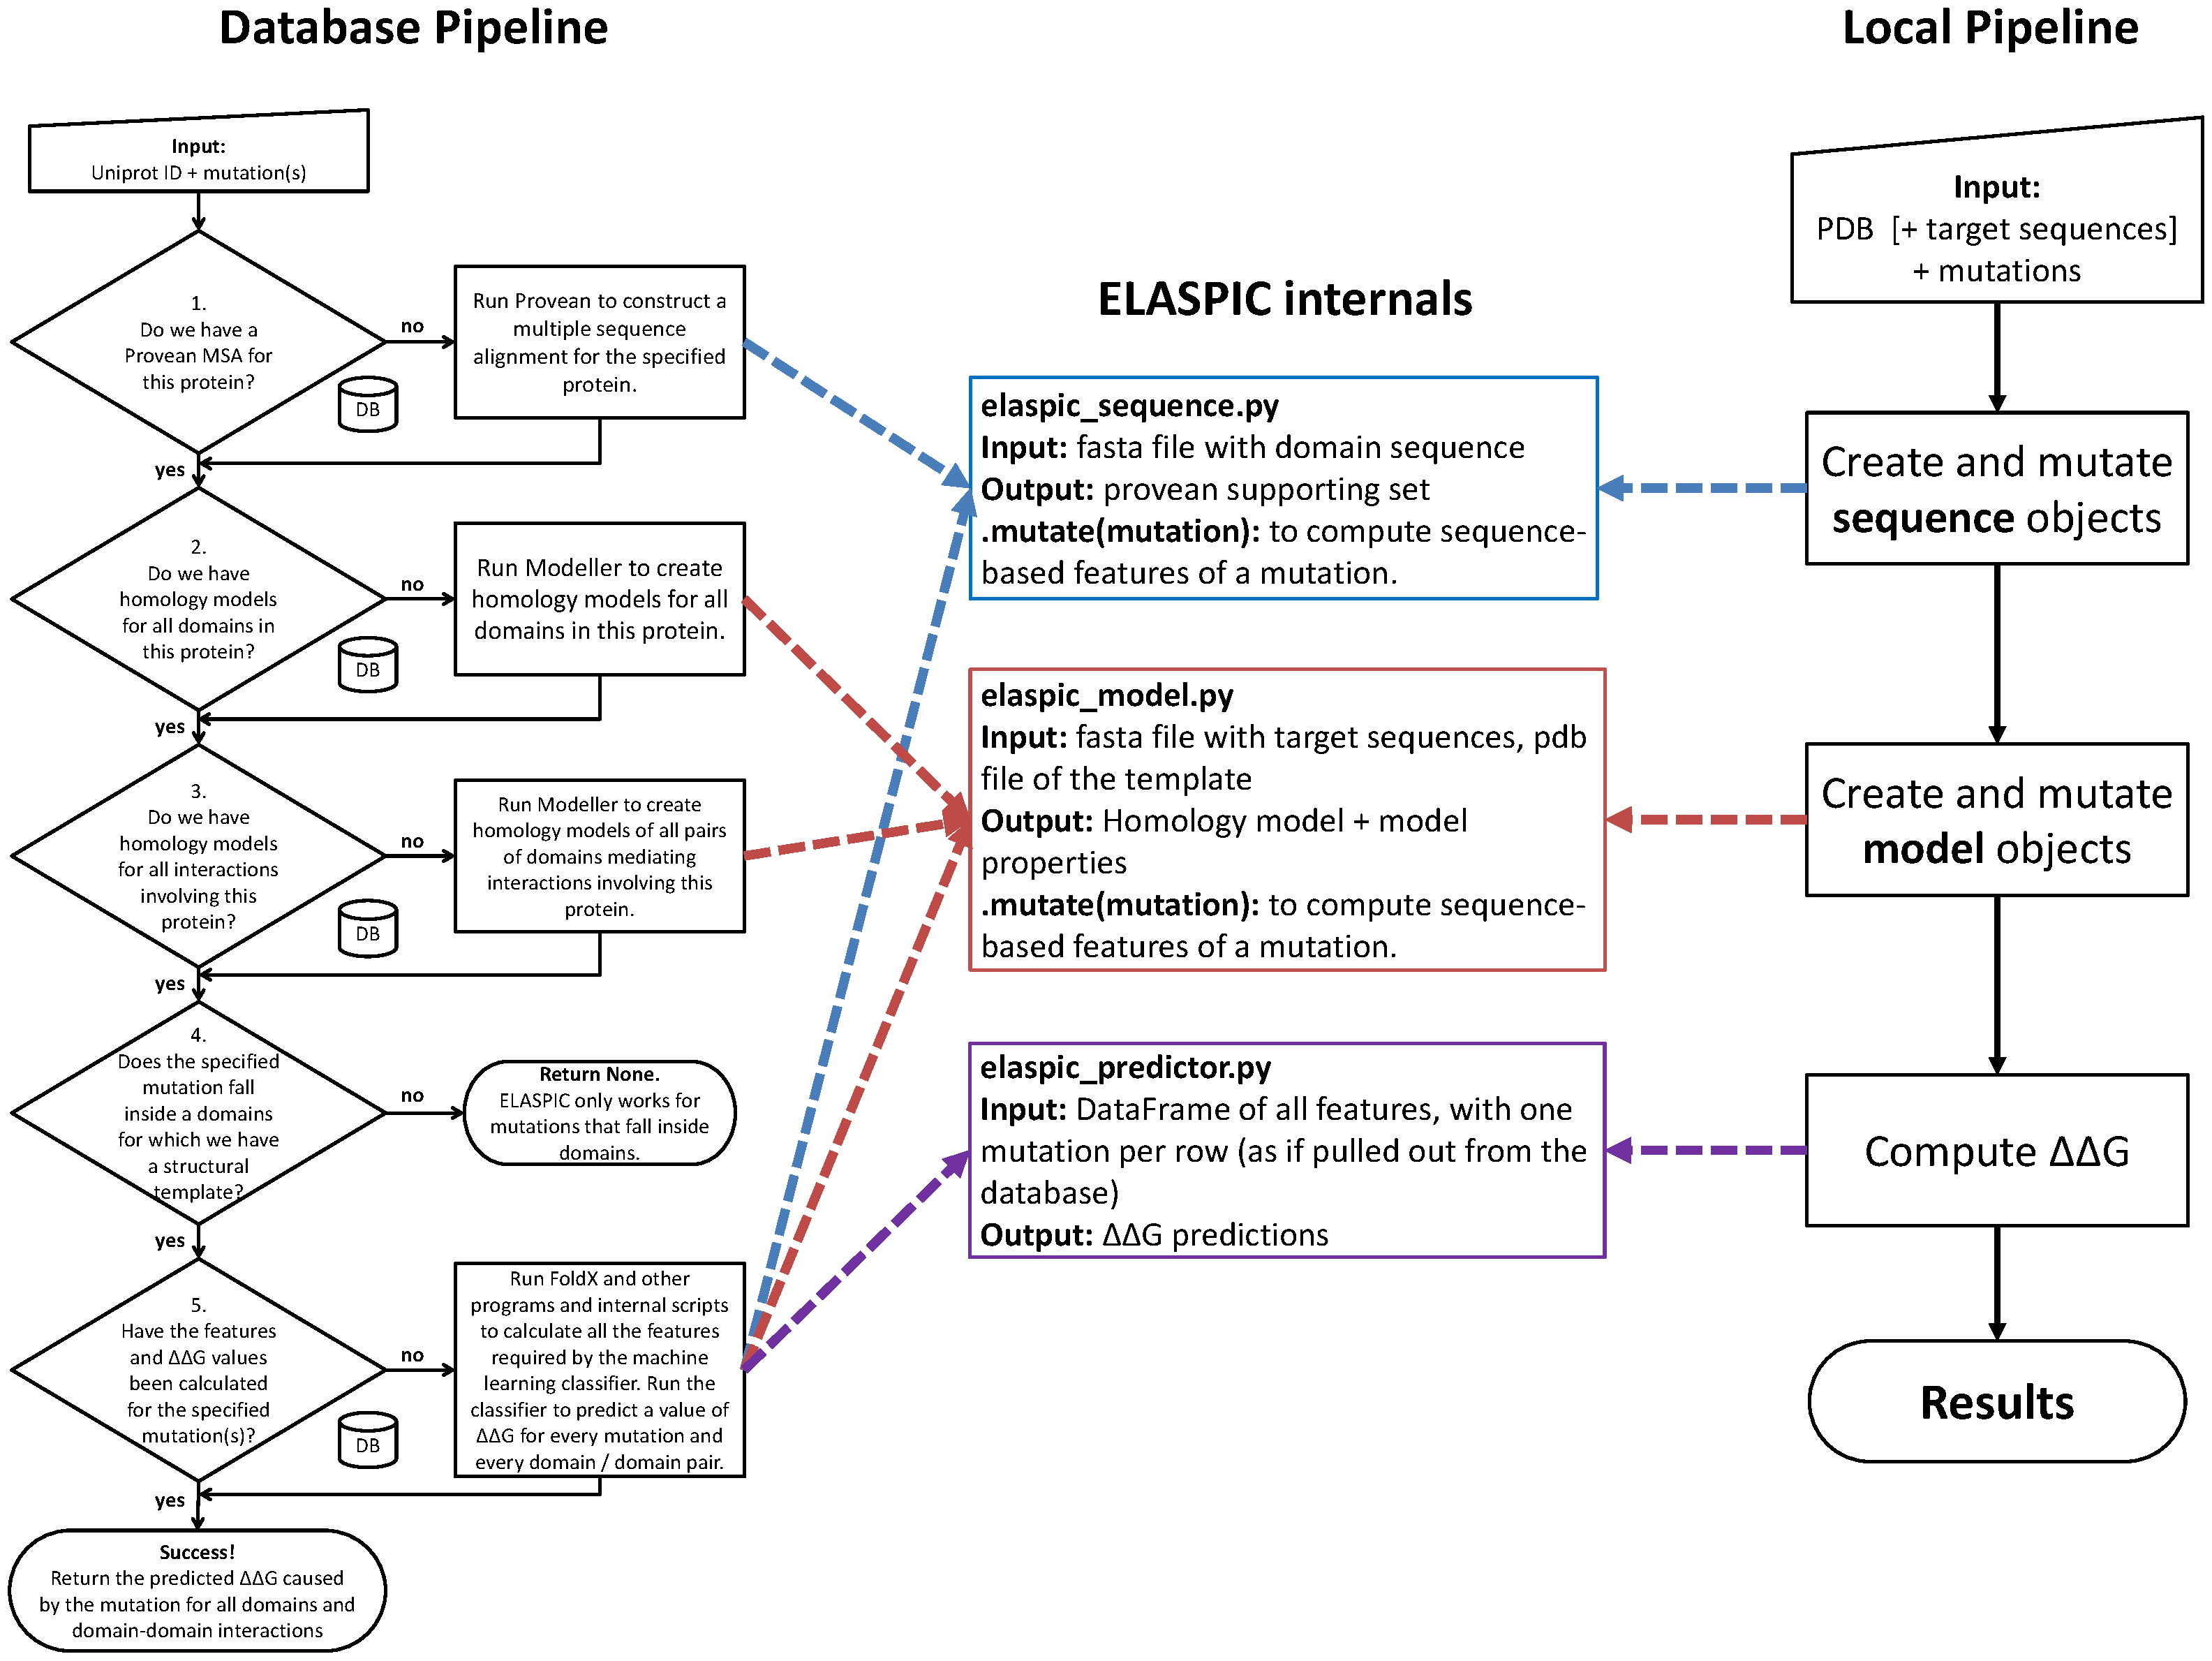
\includegraphics[width=1.0\textwidth]{static/elaspic/elaspic_flowchart.pdf}
	\caption[Overview of the ELASPIC pipeline]{Overview of the ELASPIC pipeline. A user runs the ELASPIC pipeline specifying the UniProt id of the protein being mutated, and one or more mutations affecting that protein. At each decision node, the pipeline queries the database to check whether or not the required information has been calculated previously. If the required data has not been calculated, the pipeline calculates it on the fly and stores the results in the database for later retrieval. The pipeline proceeds until homology models of all domains in the protein, and all domain-domain interactions involving the protein, have been calculated, and the $\Delta \Delta G$ has been predicted for every specified mutation.}
	\label{fig:elaspic_pipeline}
\end{figure}


\begin{figure}[ht]
	\centering
	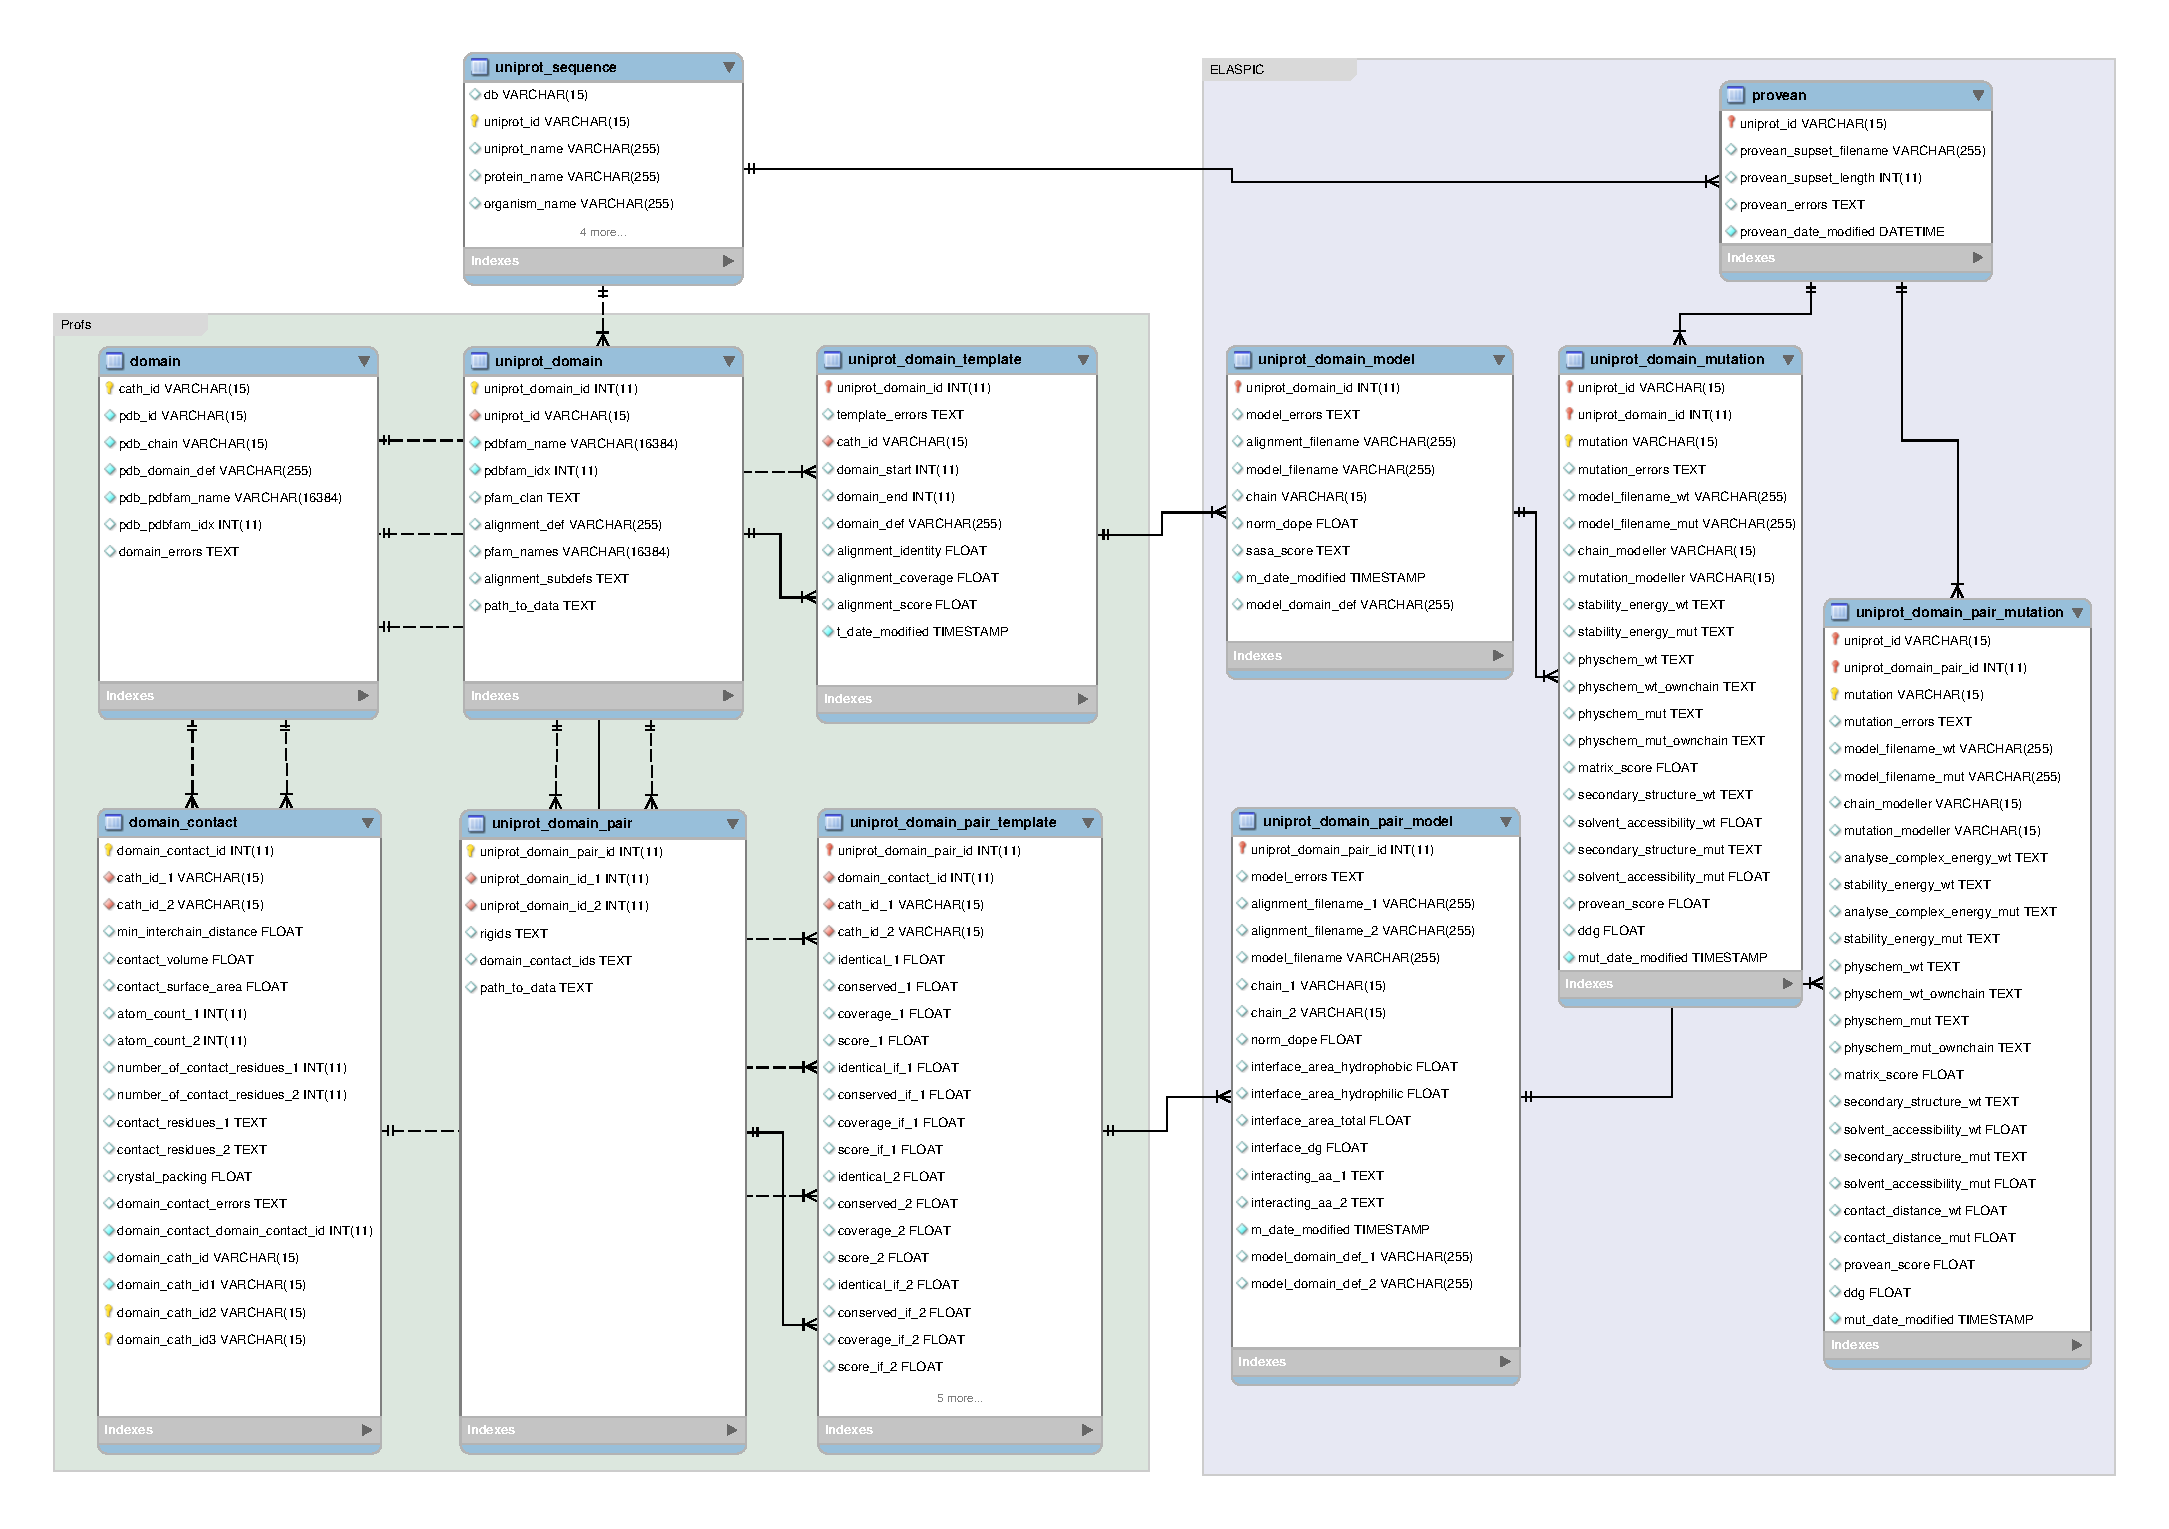
\includegraphics[width=1.0\textwidth]{static/elaspic/elaspic_schema.pdf}
	\caption{Database schema used by the ELASPIC pipeline. Tables on the green plate titled Profs are calculated using the Profs pipeline, as described in \cite{witvliet_elaspic_2016}. Tables on the purple plate titled ELASPIC are calculated using the ELASPIC pipeline, following the procedure outlined in \ref{fig:elaspic_pipeline}. A detailed description of each table can be found in \ref{tab:elaspic_database_schema}.}
    \label{fig:elaspic_database_schema}
\end{figure}


\begin{table}[ht]
\caption{ELASPIC database tables.} \label{tab:elaspic_database_schema}
\begin{tabular}{l | p{10cm}}
	\toprule
	Table name & Table description \\
	\midrule
	\textbf{domain} & Contains Profs domain definitions for all proteins in the PDB. \\
	\textbf{domain\_contact} & Contains information about interactions between Profs domains in the PDB. Only interactions that are predicted to be real by NOXclass \cite{zhu_noxclass:_2006} are included in this table. \\
	\textbf{uniprot\_sequence} & Contains protein sequences for all proteins that are annotated with Profs domains in the \textbf{uniprot\_domain} table. This table is constructed by downloading and parsing \textit{uniprot\_sprot\_fasta.gz}, \textit{uniprot\_trembl\_fasta.gz}, and \textit{homo\_sapiens\_variation.txt} files from the Uniprot. \\
	\textbf{provean} & Contains information about Provean \cite{choi_predicting_2012} supporting set files. The construction of a supporting set is the longest part of running Provean. Thus, in order to speed up the evaluation of mutations, the supporting set is precalculated and stored for every protein. \\
	\textbf{uniprot\_domain} & Contains Profs domain definitions for proteins in the \textbf{uniprot\_sequence} table. This table is obtained by downloading Pfam domain definitions for all known proteins from SIMAP \cite{rattei_simapcomprehensive_2010}, and mapping those proteins to Uniprot using the MD5 hash of each sequence. Overlapping and repeating domains are either merged or deleted, as described in \cite{witvliet_elaspic_2016}. \\
	\textbf{uniprot\_domain\_template} & Contains structural templates for domains in the \textbf{uniprot\_domain} table. The \textit{domain\_def} column contains expanded and corrected domain definitions for every domain. \\
	\textbf{uniprot\_domain\_model} & Contains information about the homology models which were created using structural templates in the \textbf{uniprot\_domain\_template} table. \\
	\textbf{uniprot\_domain\_mutation} & Contains information about the structural impact of core mutations, calculated by introducing those mutations into homology models listed in the \textbf{uniprot\_domain\_model} table. The \textit{ddg} column contains the predicted change in the Gibbs free energy of binding. \\
	\textbf{uniprot\_domain\_pair} & Contains pairs of domains that are likely to mediate the interaction between known interacting partners, obtained from Hippie \cite{schaefer_hippie:_2012} and Rolland et al. \cite{rolland_proteome-scale_2014}. \\
	\textbf{uniprot\_domain\_pair\_template} & Contains structural templates for domain pairs in the \textbf{uniprot\_domain\_pair} table. \\
	\textbf{uniprot\_domain\_pair\_model} & Contains information about homology models which were created using structural templates in the \textbf{uniprot\_domain\_pair} table. \\
	\textbf{uniprot\_domain\_pair} & Contains information about the structural impact of interface mutations, calculated by introducing those mutations into homology models listed in the \textbf{uniprot\_domain\_pair\_model} table. The \textit{ddg} column contains the predicted change in the Gibbs free energy of binding. \\
	\bottomrule
\end{tabular}
\end{table}


\section{ELASPIC predictor}

ELASPIC uses the gradient boosting of decision trees regressor (GBR). It was optimized in several ways.
\subsection{Training}

ELASPIC described in  output xxx features in total.
1. We calculated those features for the Provean and the Skempi training sets.
2. We removed features that were note different in any of the training cases (xxx for core mutations and yyy for interface mutations).

3. It has been reported that balancing the training set by including both positive and negative samples


As described in [], balancing the training set can significantly improve performance. However, with Provean balancing the training set can bias the result because most mutations are to unconserved amino acids (often alanine) and



We built two core predictors and two interface predictors:

\begin{enumerate}
	\item No sequence features but a balanced training set.
	\item Sequence features but no balanced training set.
\end{enumerate}


\begin{figure}[H]
	\centering
	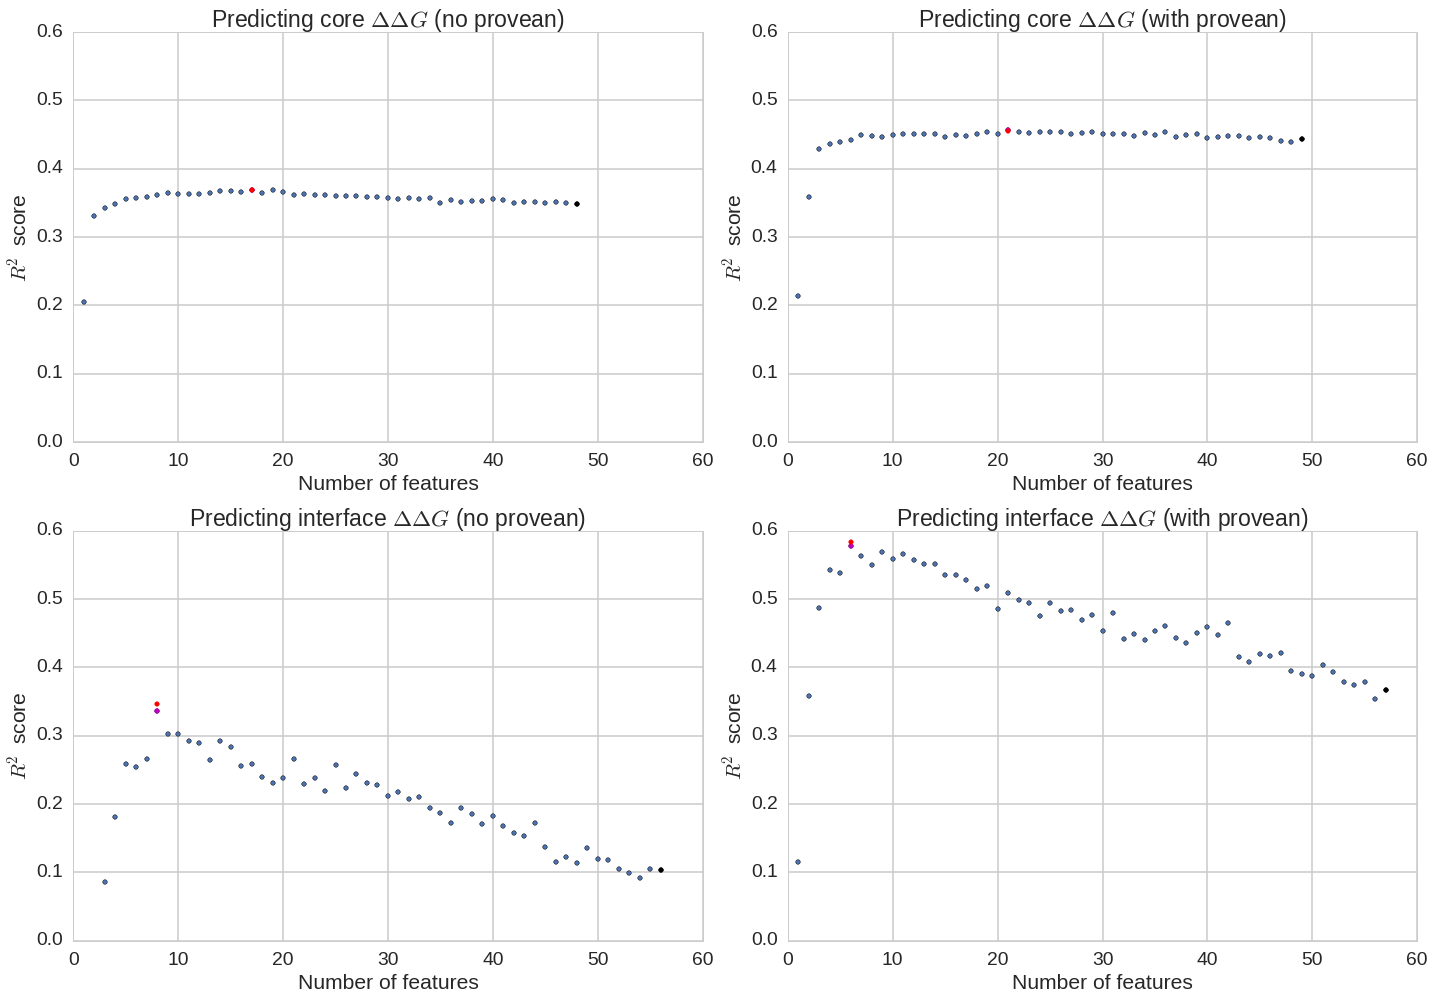
\includegraphics[scale=0.3]{image117}
	\caption{Variable elimination.}
\end{figure}

\begin{figure}[H]
	\centering
	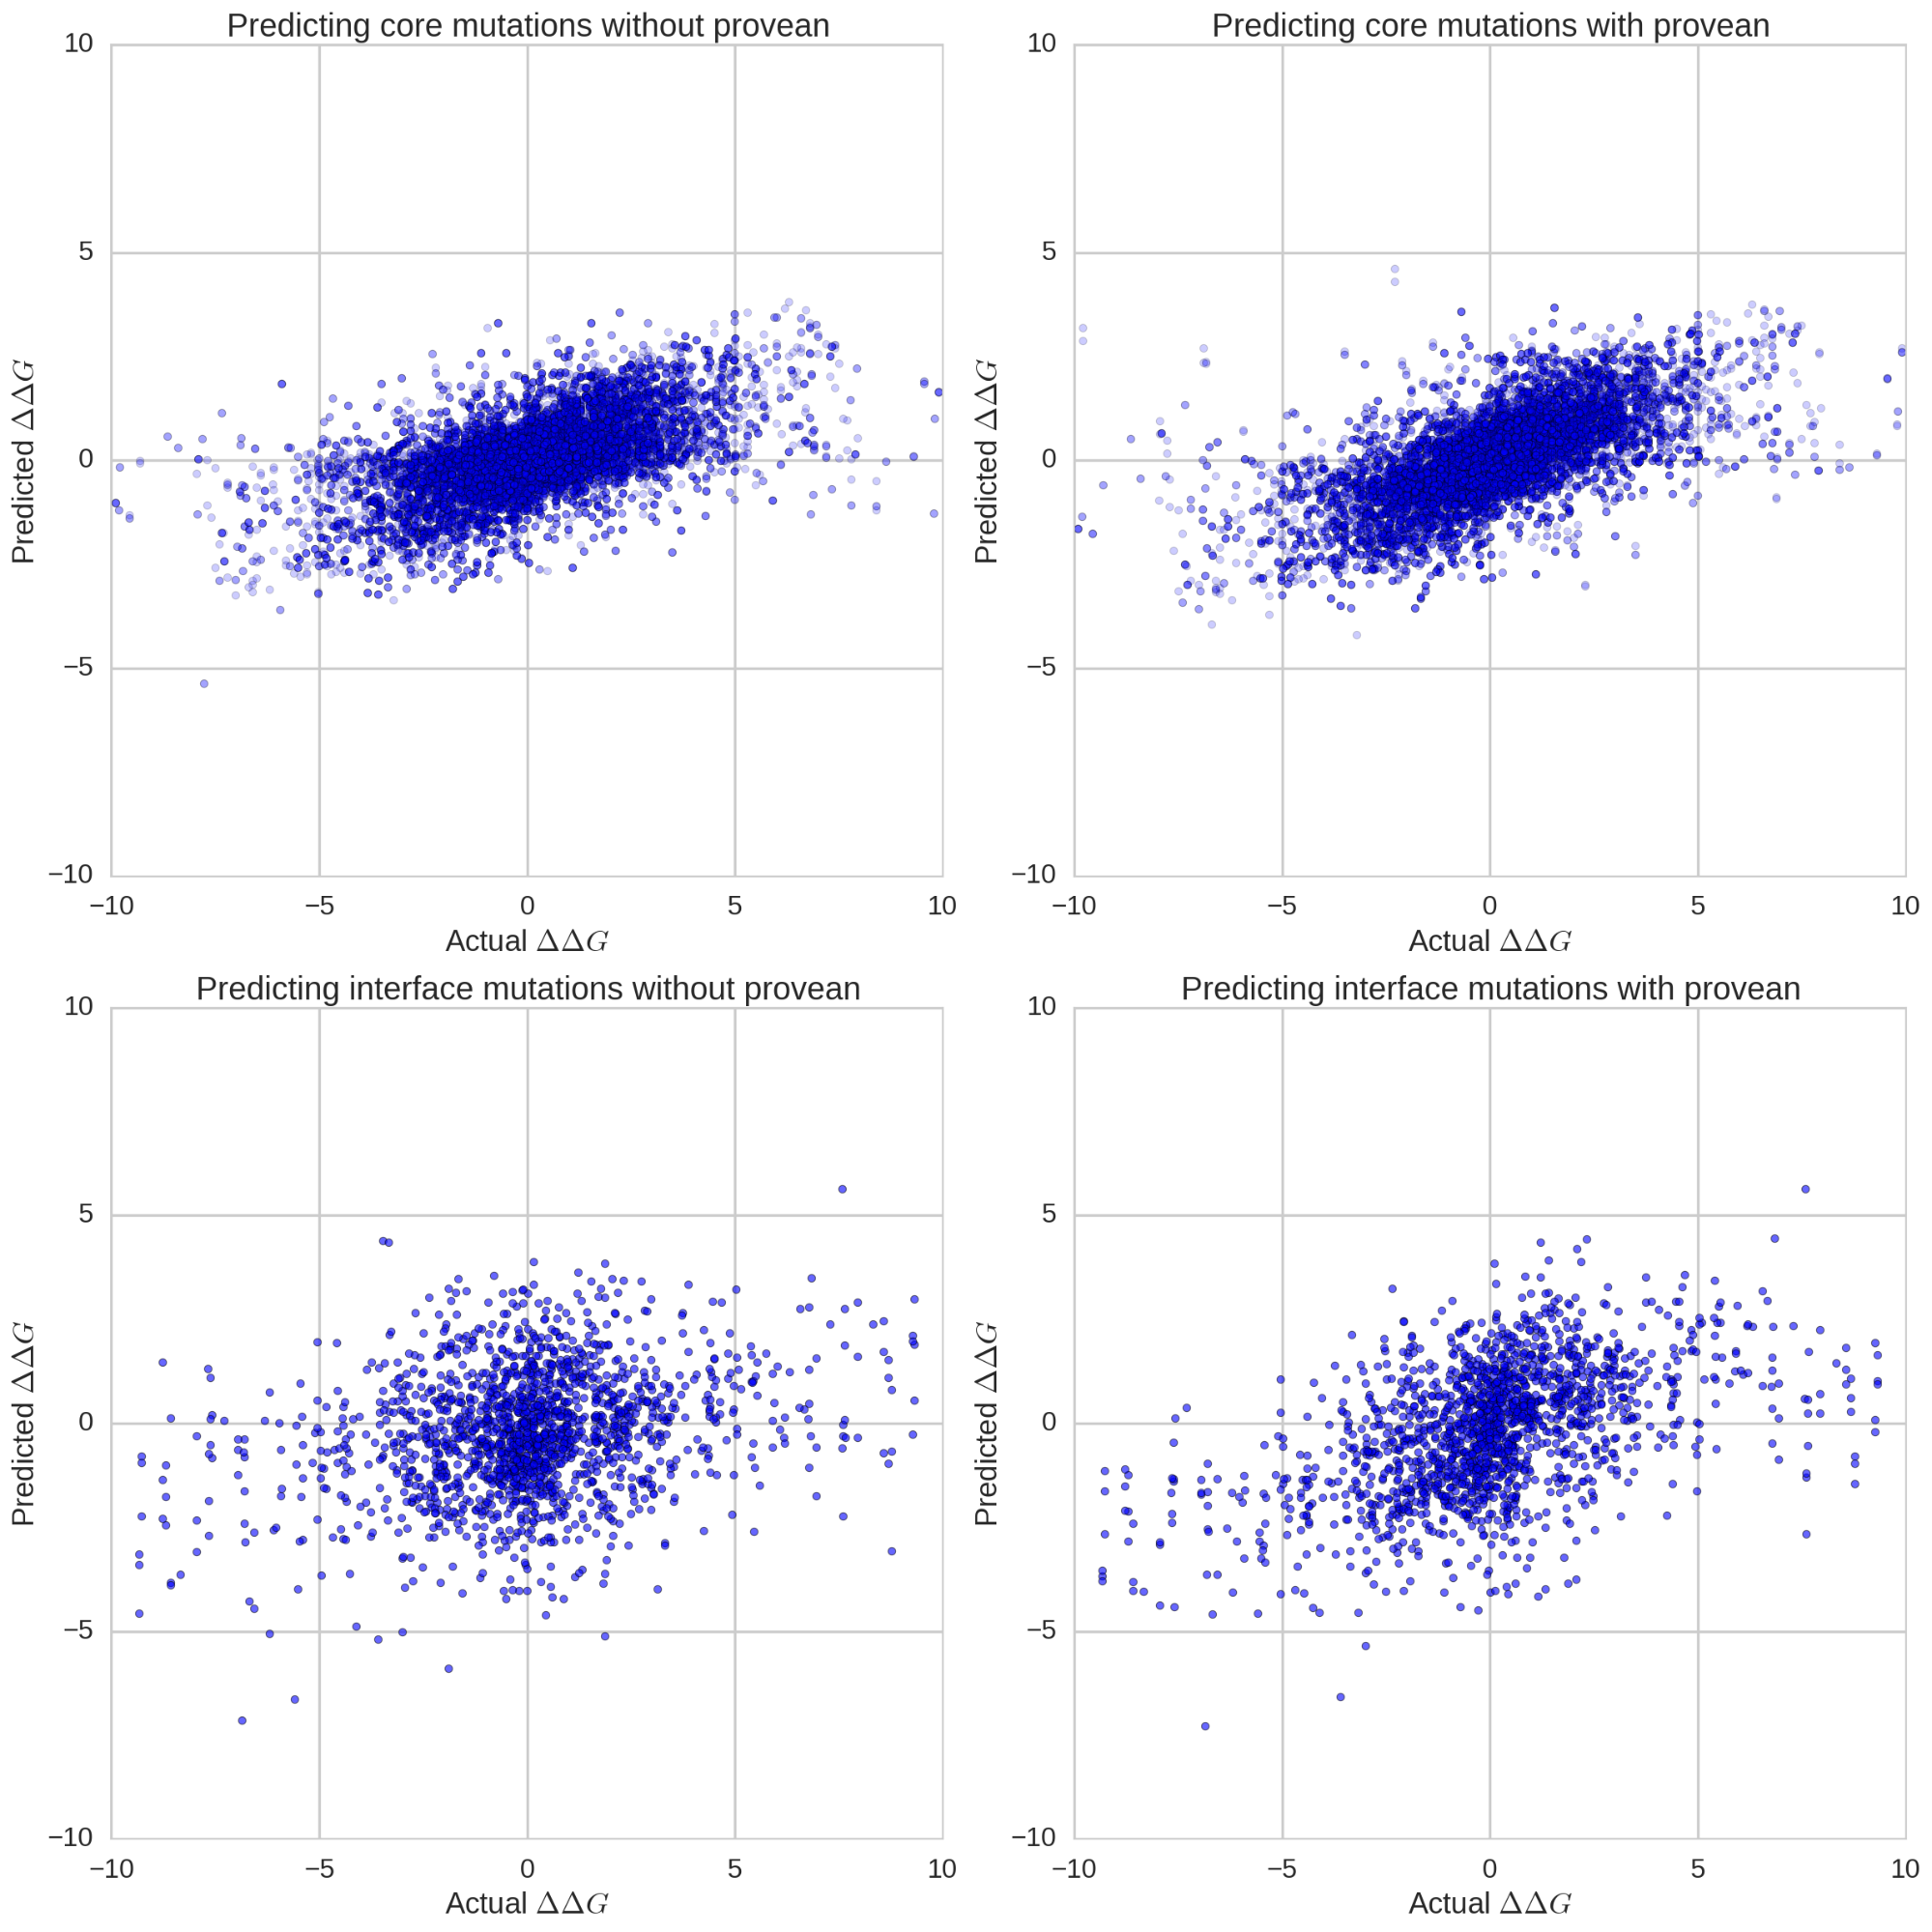
\includegraphics[scale=0.2]{image65}
	\caption{Cross-validation performance before variable elimination.}
\end{figure}

\begin{figure}[H]
	\centering
	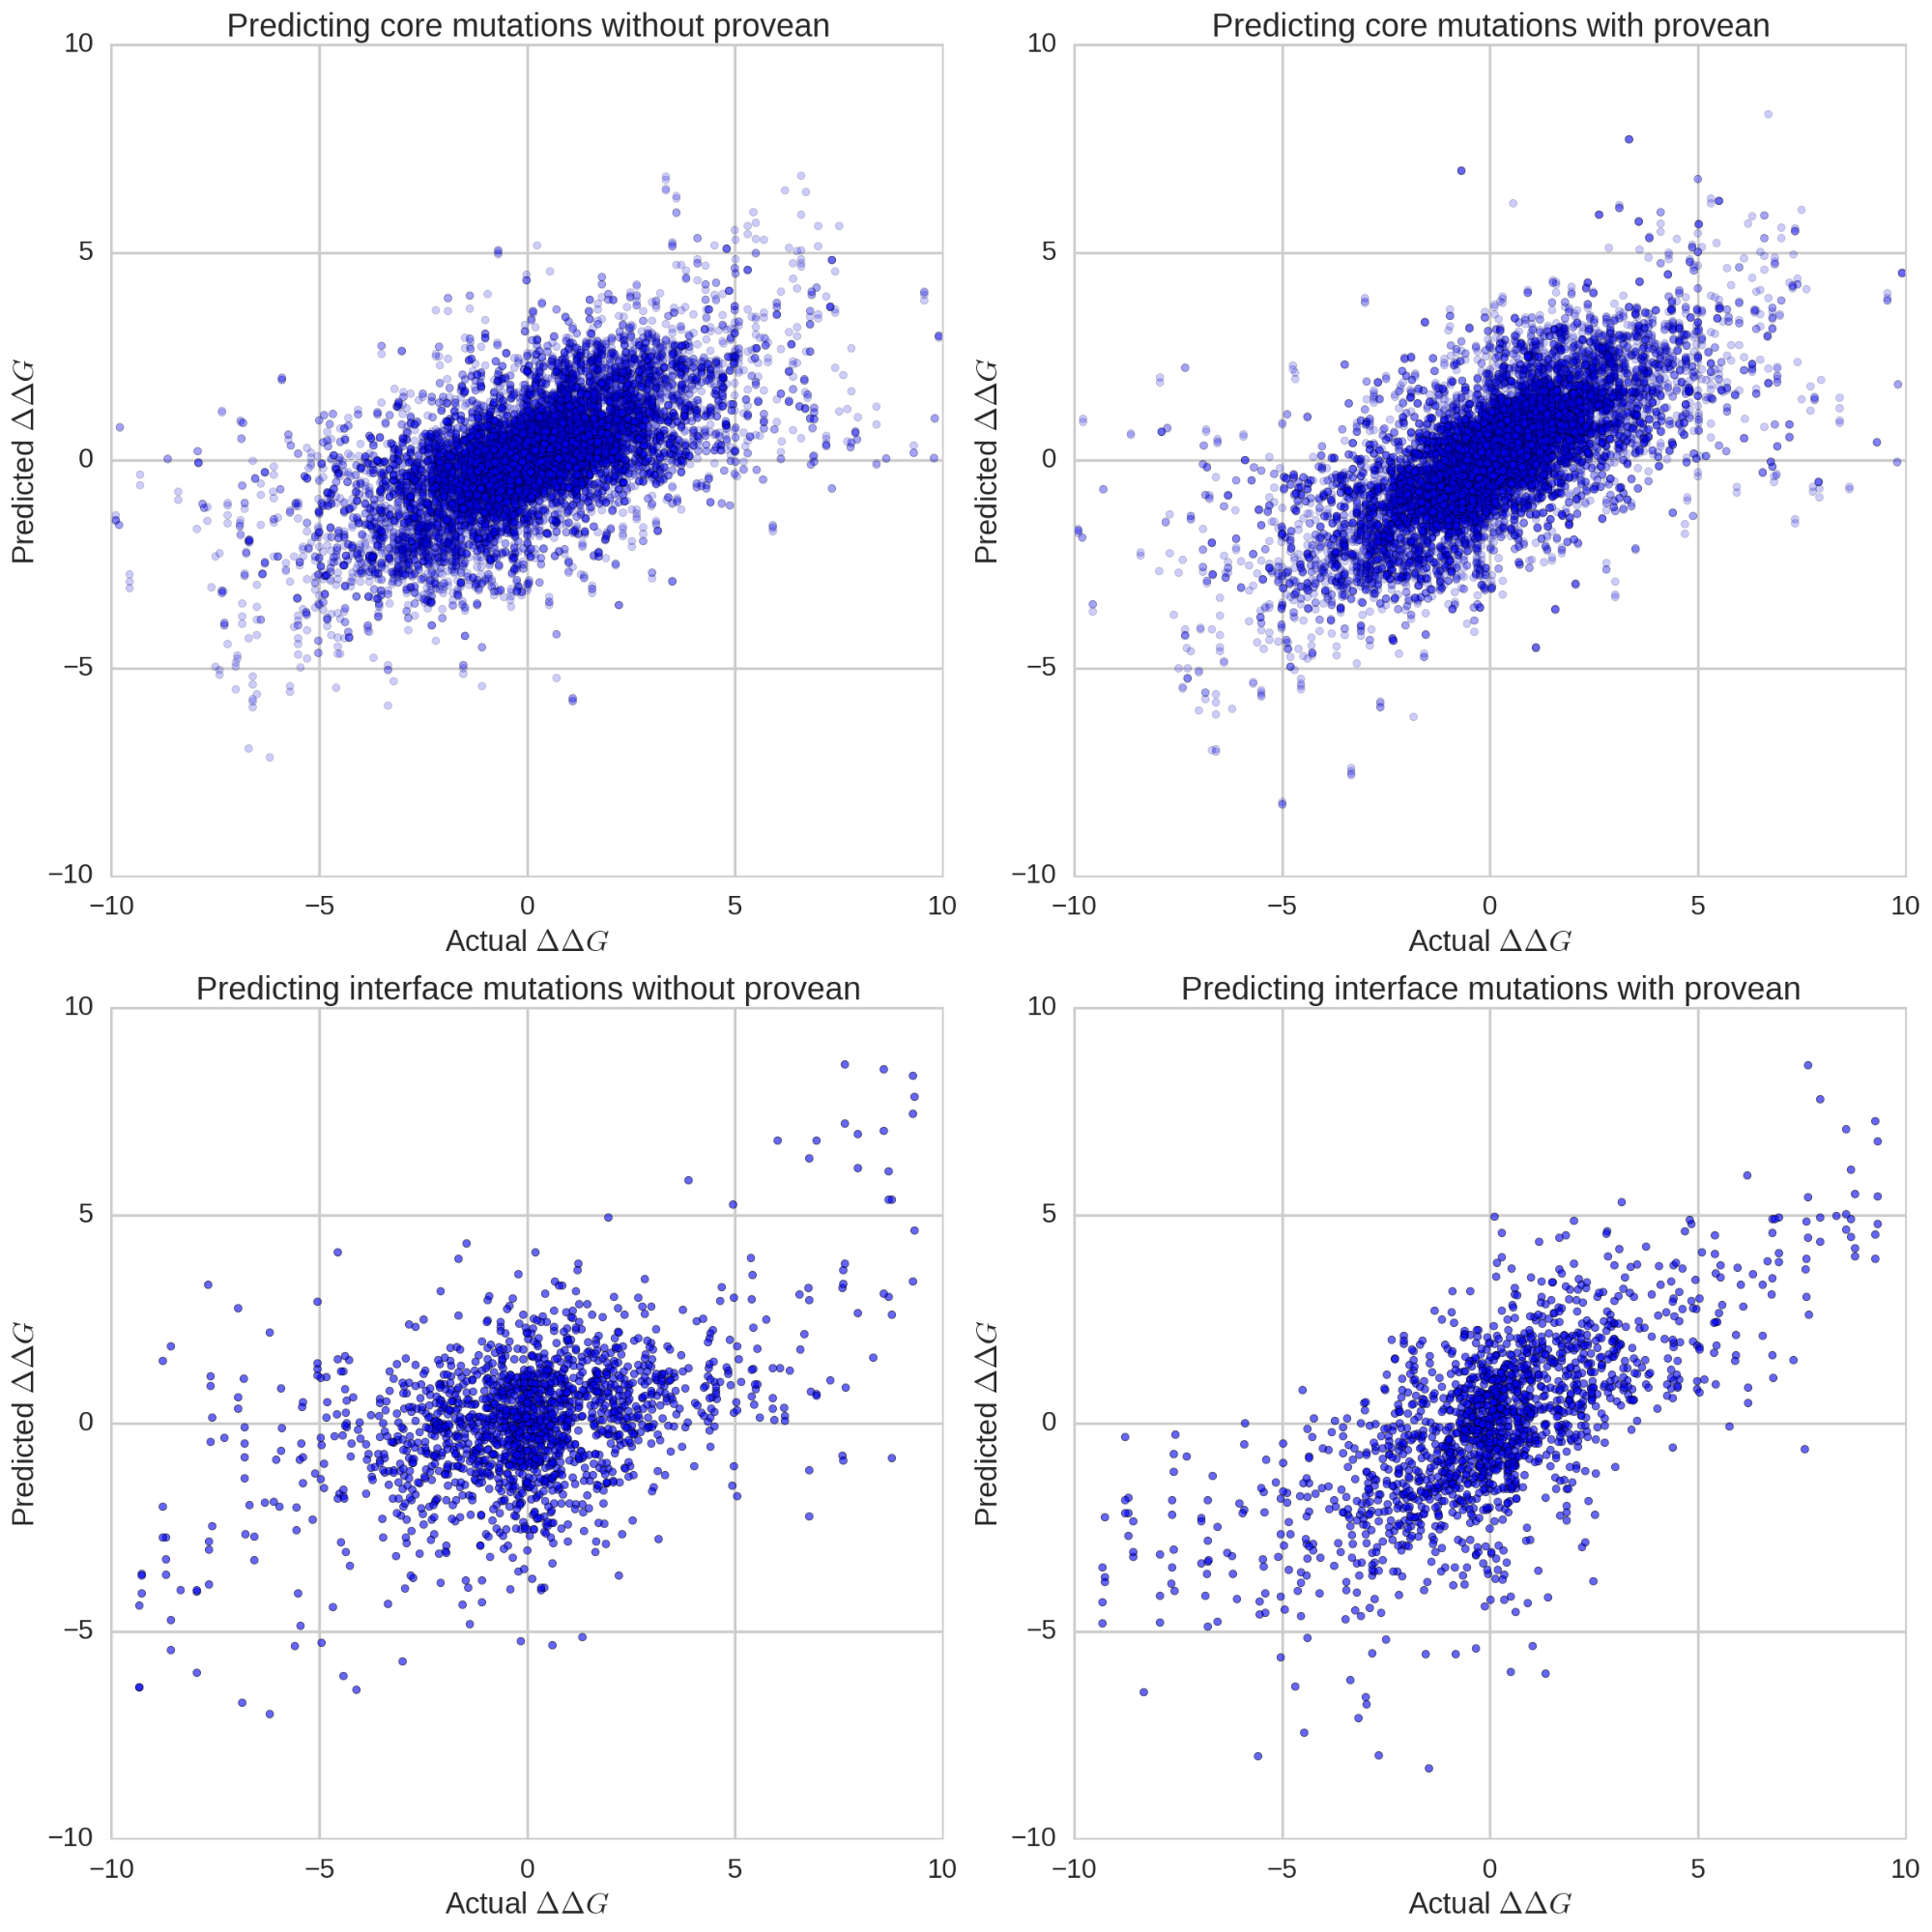
\includegraphics[scale=0.2]{image103}
	\caption{Cross-validation performance after variable elimination.}
\end{figure}

\begin{figure}[H]
	\centering
	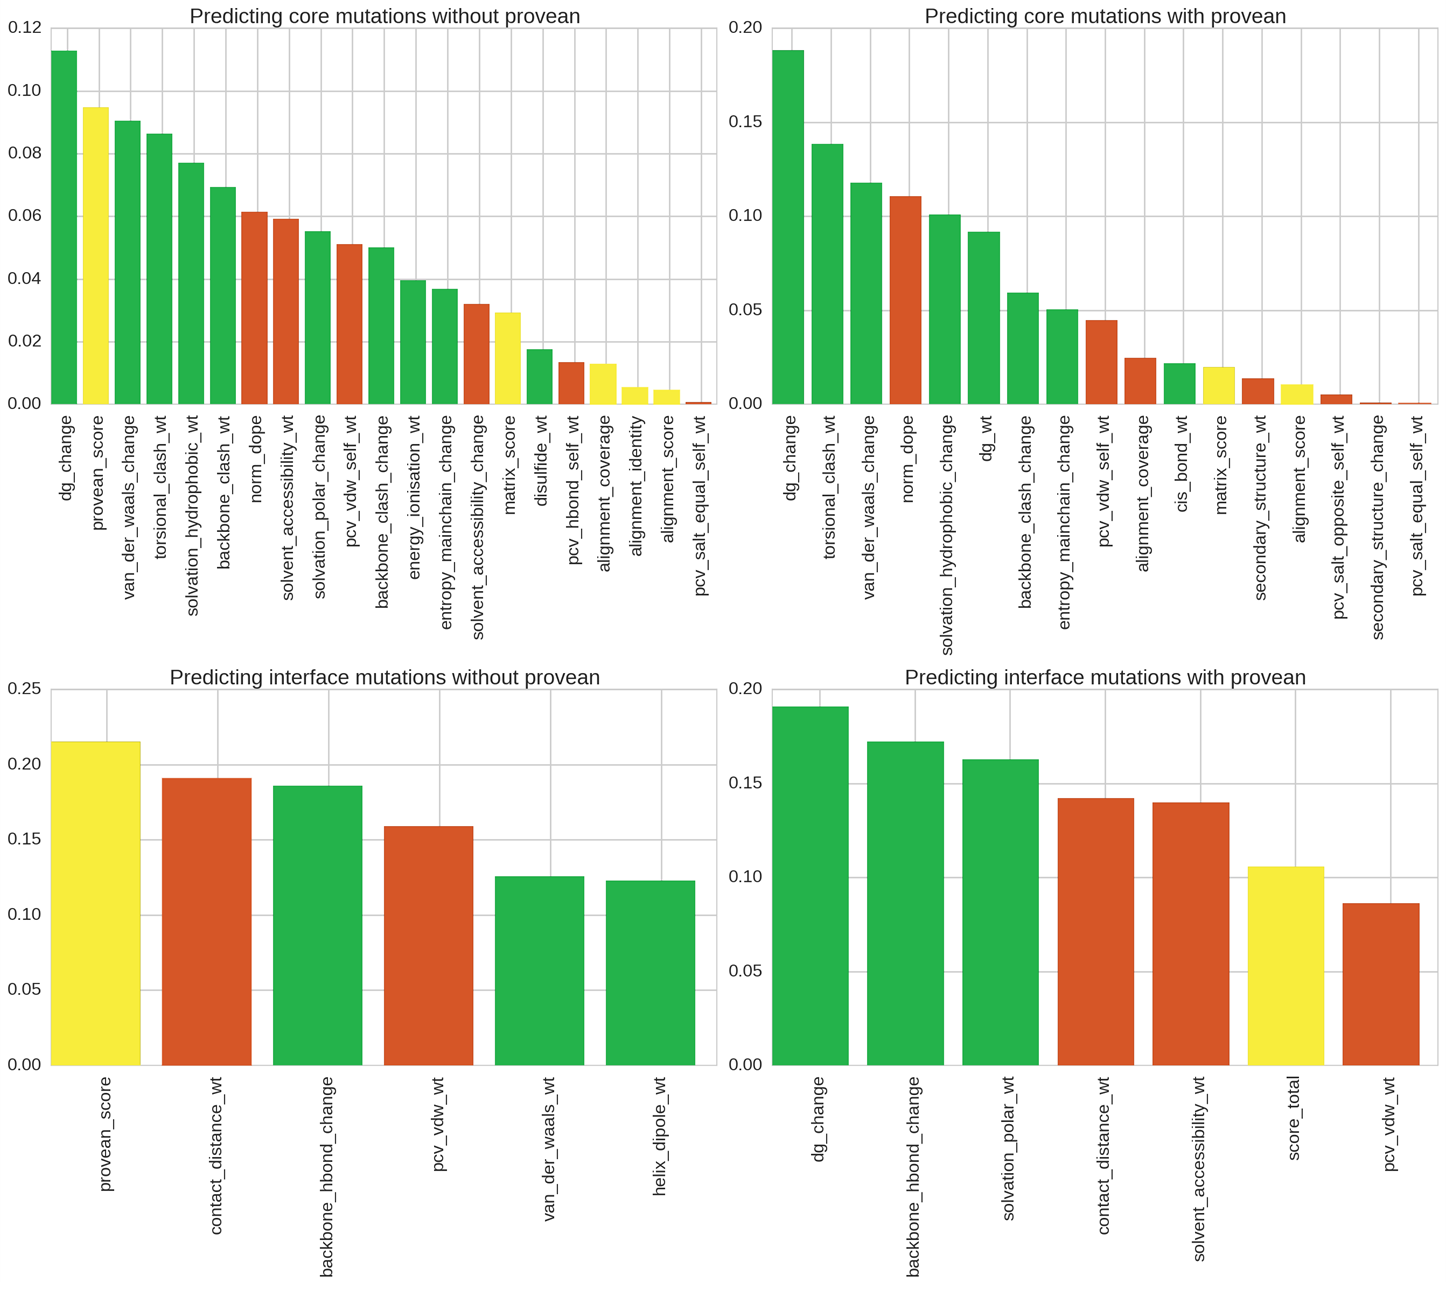
\includegraphics[scale=0.3]{image02}
	\caption{Feature importances after variable elimination.}
\end{figure}




\subsection{Validation}

Compare how well Provean, FoldX, and `ELASPIC with Provean' and `ELASPIC without Provean' distinguish between the three different datasets for both core and interface mutations.

\begin{itemize}
\item Chaperone interaction data (core mutations) \ Luciferase complementation assay (interface mutations) (use Spearman correlation coefficient).
\item Uniprot disease vs. polymorphism (use AUC / ROC / combination).
\item COSMIC driver vs. passenger.
\end{itemize}







% \subsubsection{Chaperone interaction data}
%
% \begin{figure}[H]
% 	\centering
% 	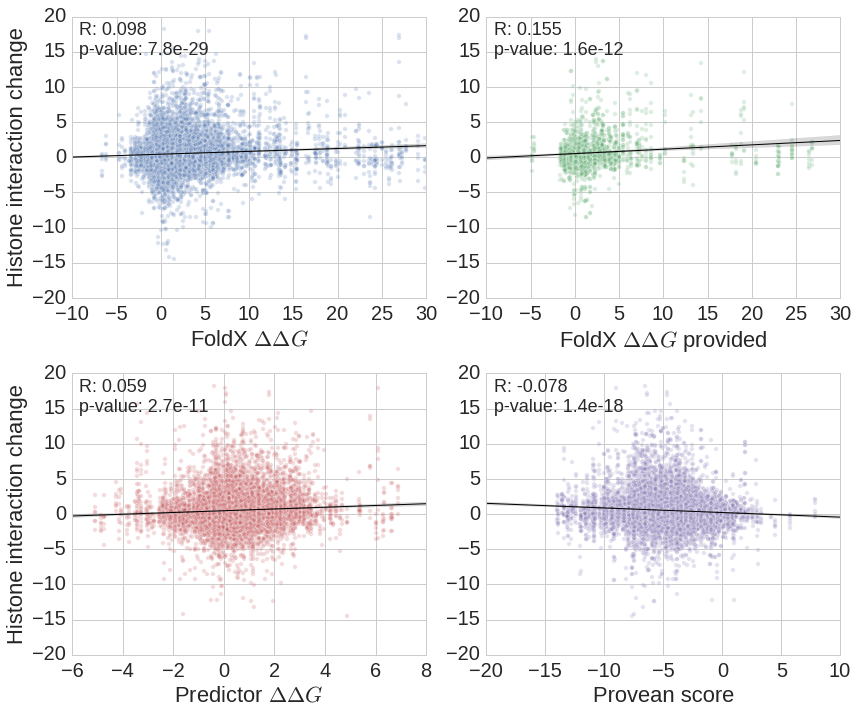
\includegraphics[scale=0.4]{image75}
% 	\caption[Core Validation]{Validation of the ELASPIC core predictor using chaperone interaction data from "Widespread Macromolecular Interaction Perturbations in Human Genetic Disorders".}
% \end{figure}
%
%
% \begin{figure}[H]
% 	\centering
% 	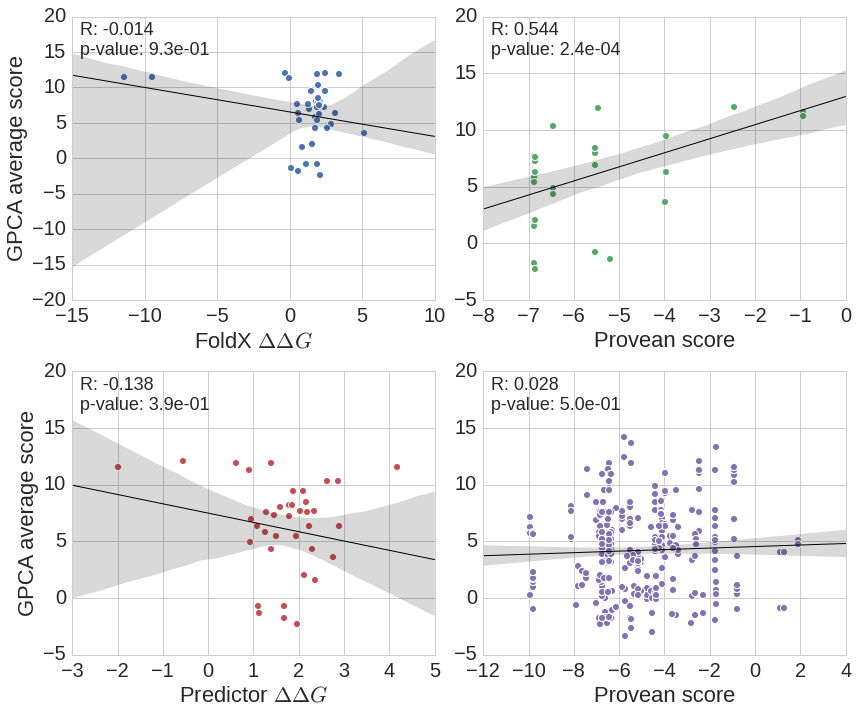
\includegraphics[scale=0.4]{image52}
% 	\caption[Interface Validation]{Validation of the ELASPIC core interface predictor using \textit{Gaussia princeps} luciferase protein complementation assay from "Widespread Macromolecular Interaction Perturbations in Human Genetic Disorders".}
% \end{figure}
%
%





\section{Structure features}

The performance of Provean is comparable to the leading mutation scoring programs, such as SITF, PolyPhen-2, Mutation Assessor, and CONDEL \cite{choi_predicting_2012}. Furthermore, Provean is distributed under a GPLv3 license, and uses \textit{supporting sets} of at most 45 sequences which can precalculated and stored. If a supporting set is available, calculating the Provean score takes several seconds per mutation.

Another widely-used mutaiton scoring tool is PolyPhen-2. It is one of the packages predicted for




\section{ELASPIC pipeline}

The ELASPIC project was started by Niklas Berliner and others in 2014 \cite{berliner_combining_2014}.

ELASPIC uses Modeller \cite{webb_comparative_2002} to construct homology models of domains and domain-domain interactions, FoldX to optimize those model and to introduce mutations \cite{schymkowitz_foldx_2005}, and the ELASPIC predictor to combine FoldX energy scores with sequence-based and other features and predict the energetic impact of a mutation on the stability of a single domain or the affinity between two domains. A flowchart describing the ELASPIC pipeline is presented in \ref{fig:elaspic_pipeline}. At each step in the pipeline, a local database is queried to see if the required information has already been calculated. If the information is available, the pipeline moves to the next step. If the information is not available, the pipeline runs the module that generates the required information, stores the generated information in the database for future access, and then moves to the next step. If the specified mutation falls outside of every domain in the protein, no predictions are returned. Otherwise, the pipeline evaluates the impact of the mutation on the stability of the domain and, if the mutation falls in a domain interface, on the affinity between two domains. In order to expedite the evaluation of mutations, we precalculated homology models and Provean supporting sets for all human proteins. Structural and sequential features, and predicted ∆∆G scores, have also been precalculated for the majority of mutations listed in the Uniprot humsavar file \cite{consortium_uniprot:_2015} and in the COSMIC \cite{forbes_cosmic:_2015} and ClinVar \cite{landrum_clinvar:_2016} databases.

Provean supporting sets, homology models and mutation ΔΔG scores are available from the ELASPIC
downloads page: \url{http://elaspic.kimlab.org/static/download/}. The source code of the python package implementing the ELASPIC pipeline is available from \url{https://github.com/kimlaborg/elaspic}, and the documentation for the ELASPIC pipeline can be accessed online at \url{http://elaspic.readthedocs.org/}.

\section{Homology modelling of the human proteome}

\begin{figure}[H]
	\centering
	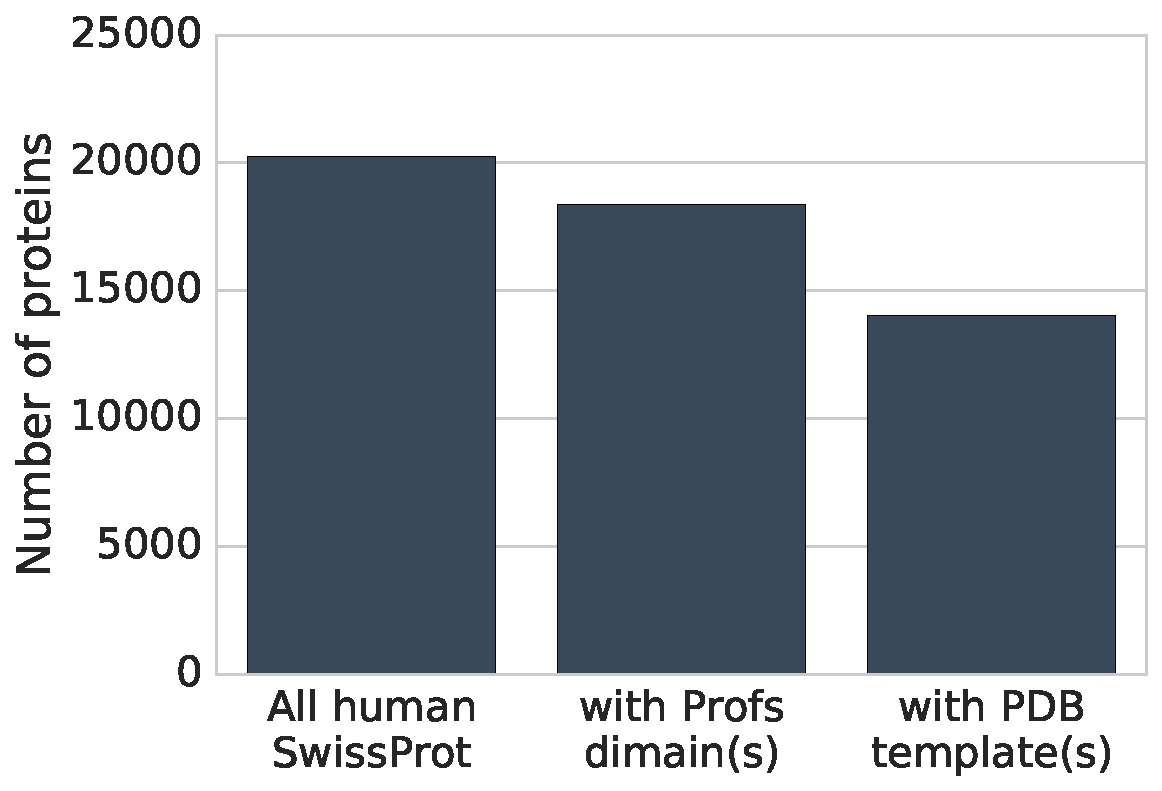
\includegraphics[scale=0.3]{elaspic_statistics/missing_template}
	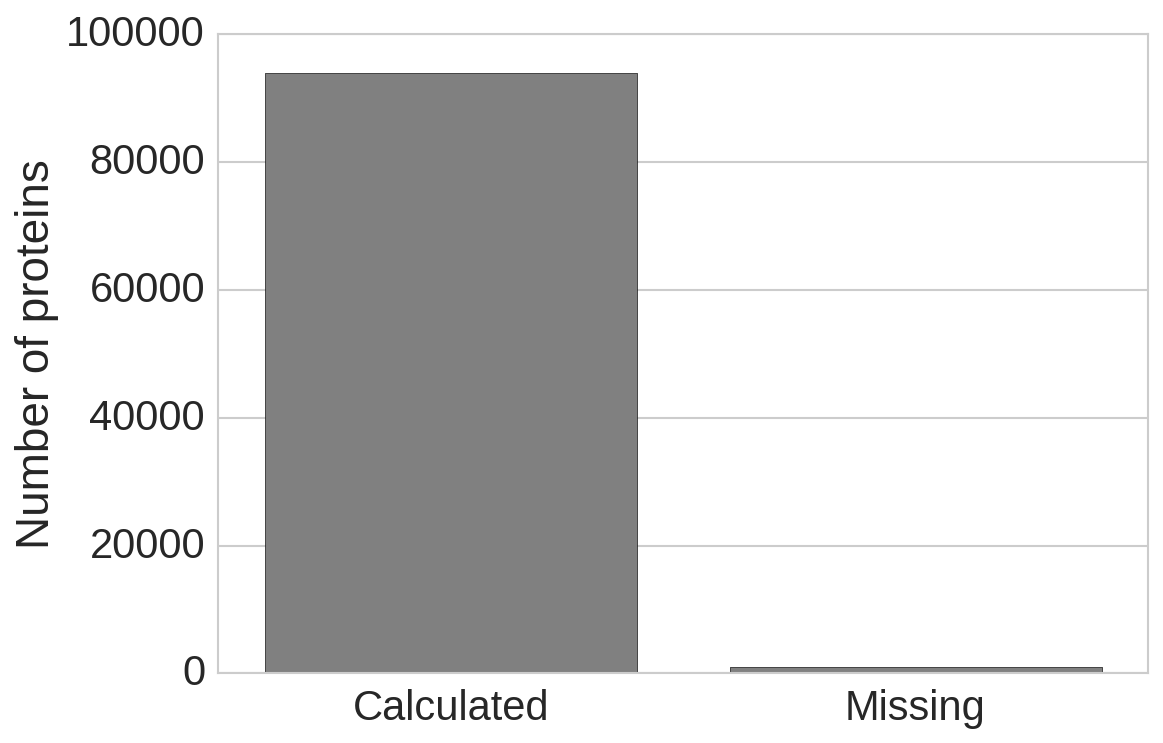
\includegraphics[scale=0.3]{elaspic_statistics/missing_model_protein}
	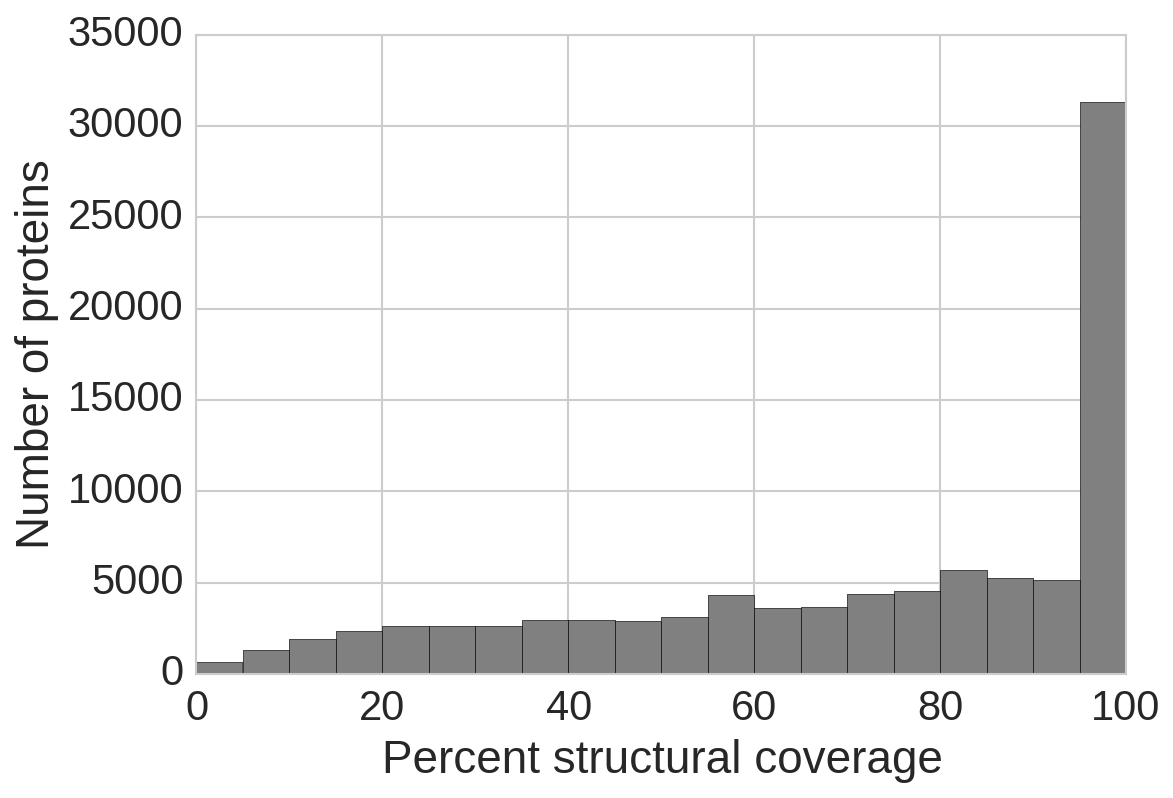
\includegraphics[scale=0.3]{elaspic_statistics/structural_coverage_hist}
	\caption{\textbf{Left}: statistics of how many homology models we were able to calculate. \textbf{Right}: structural coverage for proteins with at least one domain with a structural model.}
\end{figure}



\section{ELASPIC web service}

\begin{table}[H]
	\centering
	\caption{ELASPIC web service API.}
	\label{my-label}
	\begin{tabular}{lll}
	\textbf{Method} & \textbf{HTTP request} & \textbf{Description} \\
	submitjob & POST /submitjob & Submit a job to be run on a SGE cluser. \\
	jobstatus & GET /submitjob & View the results of a job.
	\end{tabular}
\end{table}



\section{Training sets}

\subsection{Core}

Sanhi et al. databaset (taipale)

\subsection{Interface}
